\documentclass[10pt]{article}
\usepackage[usenames]{color} %used for font color
\usepackage{amssymb} %maths
\usepackage{fancyvrb}
\usepackage{amsmath} %maths
\usepackage[utf8]{inputenc} %useful to type directly diacritic characters
\usepackage[letterpaper, portrait, margin=1in]{geometry}
\usepackage{graphicx,wrapfig}
\usepackage{booktabs}
\usepackage{multicol}
\begin{document}
\subsection*{MSDS650 Week 7 Unsupervised Learning Assignment - Nathan Worsham}
According to David Epstein (n.d.), statistical clustering "refers to several related problems: partitioning a set of input points into a fixed number of "closely related" subsets; finding a small number of representative center points; or matching the point distribution to a family of overlapping continuous distributions.” Whereas unsupervised learning is “used to draw inferences from datasets consisting of input data without labeled responses” (Mathworks.com, 2015). Unsupervised learning uses clustering--though it also uses other methods--to try to identify patterns or groups in the data.\\
Packages in R for performing unsupervised learning:\\
randomUniformForest - https://cran.r-project.org/web/packages/randomUniformForest/
randomUniformForest.pdf\\
autoencoder - https://cran.r-project.org/web/packages/autoencoder/autoencoder.pdf\\
bgmm - https://cran.r-project.org/web/packages/bgmm/bgmm.pdf\\
cclust - https://cran.r-project.org/web/packages/cclust/cclust.pdf\\
som - https://cran.r-project.org/web/packages/som/som.pdf\\
The measures of quality of the learning algorithm you would expect to see for unsupervised learning gets a bit trickier. Whereas with supervised learning you have a training set, so a portion of this can be held back to test the performance but with unsupervised there is no such training set. I think in this case it depends on what is being classified, for example if it is something where someone has domain knowledge then that person could hand label some data as a “gold standard” to compare against—comparing accuracy of the model's predictions. With my example, I find the “eye-test” seemed to be the best--meaning what looked the best. I chose to work with data for the top 50 quarterbacks in the NFL up through week 12. When I was trying to decide how many clusters to have the quarterbacks separated into, after plotting several clusters, it seemed obvious that there were 3 distinct tiers and that 4, 5 (and even up to 10) were too many levels.\\
\subsection*{Example}
As I mentioned above, I chose for my example to use the same kmeans exercise as was given with the assignment as an example but exploring NFL quarterback statistics with it. First I needed to change my data to only numeric as kmeans does not appear to work with anything else. I elected to move the player names to the rownames of the dataframe and then removed the team and position column:
\begin{verbatim}
setwd("/Users/worshamn/Dropbox/Documents/Regis/MSDS650/week7/")
passing <- read.csv("nflpassing_names.csv",sep = '\t')
playernames <- passing[,1]
passing <- passing[,-1]
rownames(passing) <- playernames
#remove team and postition
passing <- passing[,-2]
passing <- passing[,-2]
> head(passing)
              Rk Comp Att  Pct Att.G  Yds Avg Yds.G TD Int X1st X1st. Lng X20 X40 Sck  Rate
Tom Brady      1  294 451 65.2  41.0 3600 8.0 327.3 28   4  172  38.1  76  43  10  25 106.7
Philip Rivers  2  317 463 68.5  42.1 3511 7.6 319.2 23   8  169  36.5  70  38   6  26 100.1
Carson Palmer  3  241 378 63.8  34.4 3337 8.8 303.4 27   9  161  42.6  64  49  10  17 105.9
Matt Ryan      4  286 434 65.9  39.5 3212 7.4 292.0 16  12  161  37.1  55  34   6  20  88.6
Drew Brees     5  282 414 68.1  41.4 3200 7.7 320.0 20  10  144  34.8  80  45   9  25  97.1
Eli Manning    6  274 435 63.0  39.5 3021 6.9 274.6 23   9  144  33.1  87  36   8  18  92.5
\end{verbatim}
I ran through different numbers of clusters and then plotted to get an idea of what a good clustering number should be. I chose at first to always use passer rating on the x-axis as that is a summary number intended to incorporate all of the other player data into one number. In this particular list, the players are ranked 1 to 50 by most yards. So viewing yards versus rating gives a good picture of the clusters:
\begin{verbatim}
km <-kmeans(passing[,1:17], 3)
plot(passing[,17], passing[,6], col=km$cluster, xlab = 'rating',ylab = 'yards')
\end{verbatim}
Picture of the 3, 4, 5, and 10 clusters:
\par
\raisebox{-.6\height}{
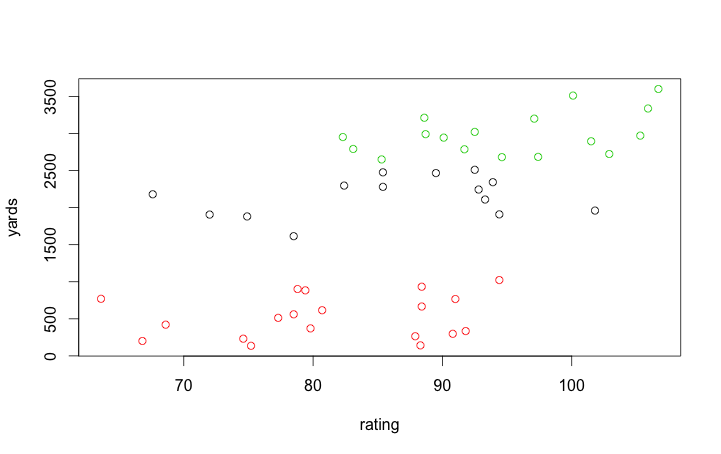
\includegraphics[width=8cm]{yardsVsRating.png}}%
\hfill
\raisebox{-.6\height}{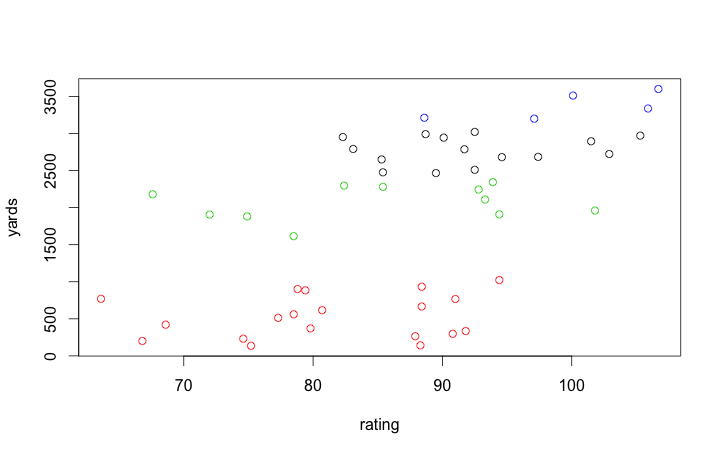
\includegraphics[width=8cm]{yardsVsRating4Clust.png}}%
\par
\par
\raisebox{-.6\height}{
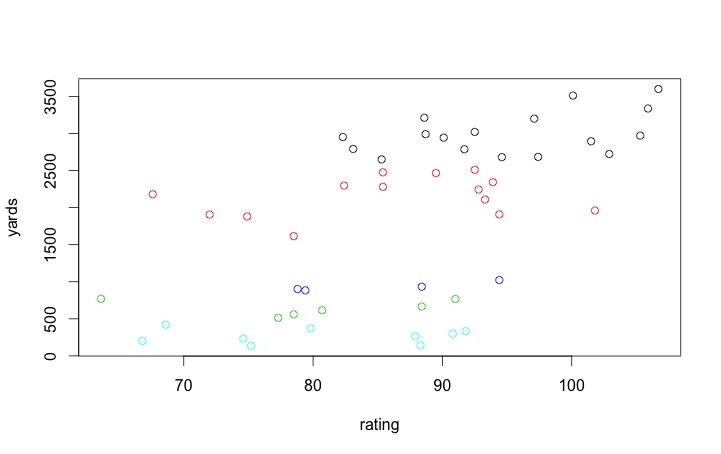
\includegraphics[width=8cm]{yardsVsRating5Clust.png}}%
\hfill
\raisebox{-.6\height}{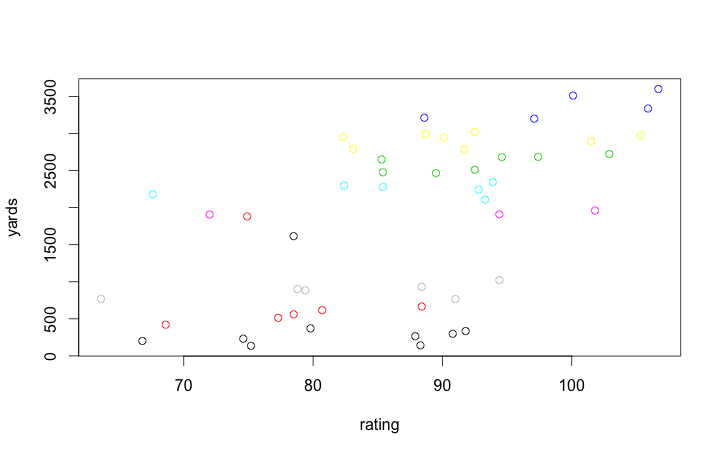
\includegraphics[width=8cm]{yardsVsRating10Clust.png}}%
\par
4 doesn't seem too bad having a top tier with 5 elite players, but it is strange that this group disappears when it moves to 5 clusters. It really seemed like there was a natural 3 group break. I then began trying many different statistics against each other. The thing I found most interesting is that seeing the original cluster places a context in your mind and then when viewing other stats where the group clustering is very muddy, you can still pick out the 3 groups and see how they relate. An example of this is Completion Percentage versus Rating and versus Ranking:
\par
\raisebox{-.6\height}{
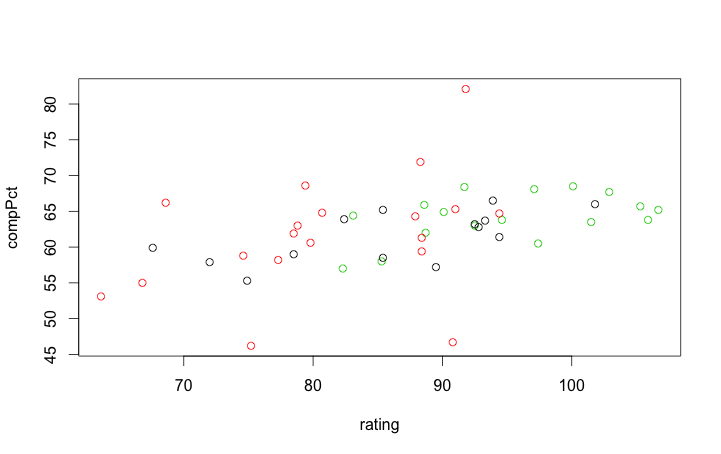
\includegraphics[width=8cm]{compPctVsRating.png}}%
\hfill
\raisebox{-.6\height}{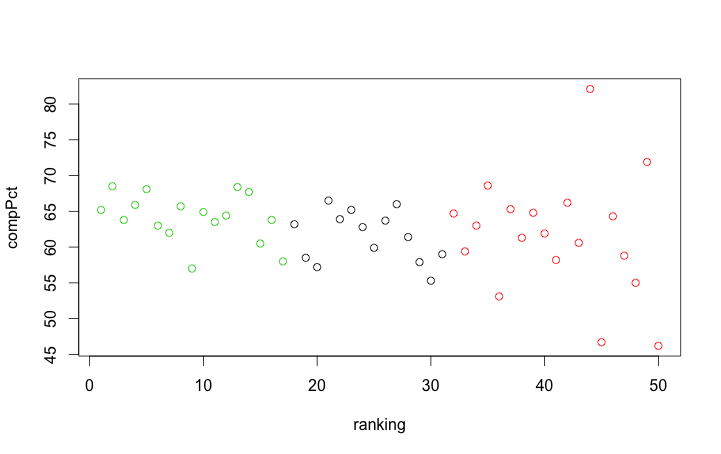
\includegraphics[width=8cm]{compPctVsRanking.png}}%
\par
Here we see the groups mixed together on the versus Rating graph but because of the previous knowledge of the 3 groups we still get an idea how those groups relate. We can see that some players with not a lot of yards--therefore lower ranked--have a decent passer rating and completion percentage, some even have better stats than the top tier. When we look at it instead against Ranking the groups separate again. In this graphic we can see that the tier 1 and 2 groups have less variation in Completion Percentage compared to the tier 3 group.
\par Other interesting things I found is that First Downs with how they relate to Yards and Touchdowns clearly follow what looks like a straight line indicating a strong relationship:
\pagebreak
\par
\raisebox{-.6\height}{
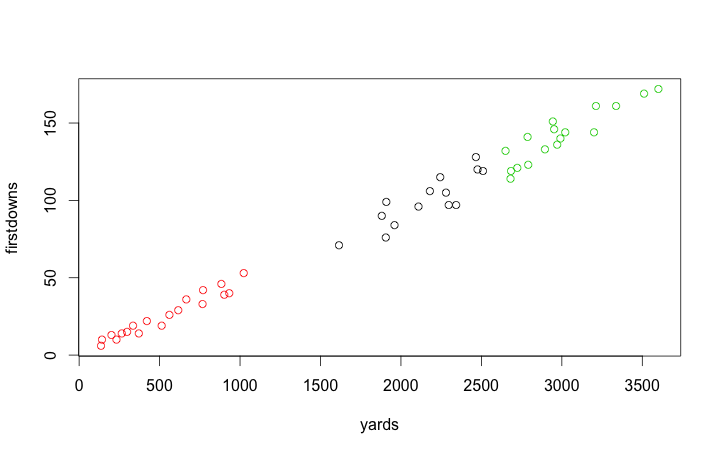
\includegraphics[width=8cm]{firstdownsVsYards.png}}%
\hfill
\raisebox{-.6\height}{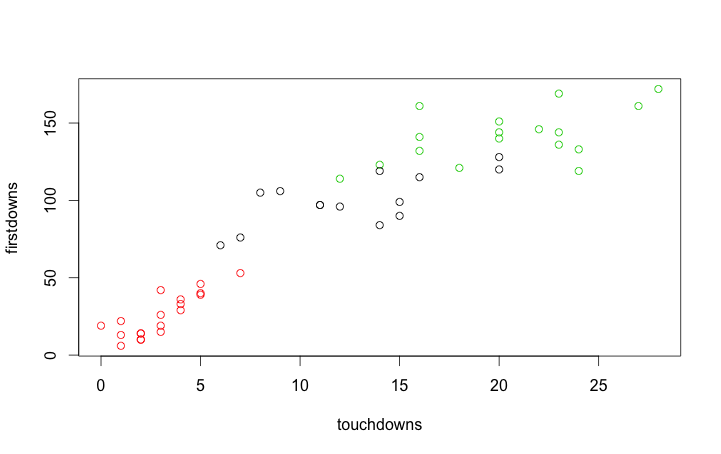
\includegraphics[width=8cm]{firstdownsVsTouchdowns.png}}%
\par
But then not so much versus Sacks or Rating:
\par
\raisebox{-.6\height}{
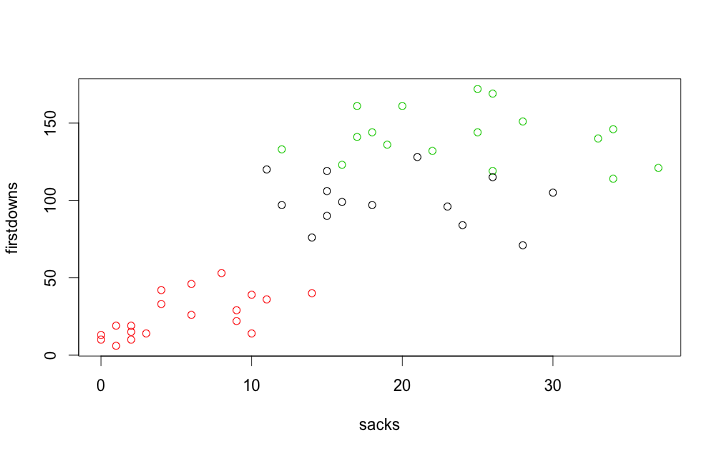
\includegraphics[width=8cm]{firstdownsVsSacks.png}}%
\hfill
\raisebox{-.6\height}{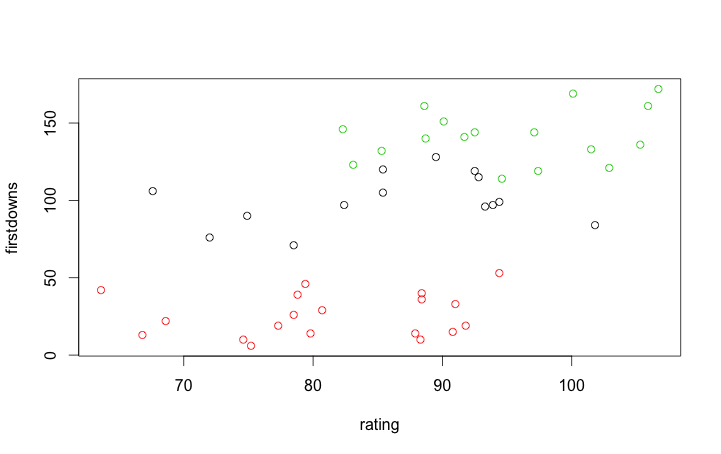
\includegraphics[width=8cm]{firstdownsVsRating.png}}%
\par
What is also interesting about First Downs on these 4 figures is that the 3 group tier stays quite separated from each other.
\par Another interesting find is that there appears to be a correlation between Passer Rating and having a higher number of Attempts. Of course a high number of Completions would correlate as well, but it would seem to get a high Passer Rating a lot of Attempts need to be made. And again the 3 tiers stay separated nicely:
\par
\raisebox{-.6\height}{
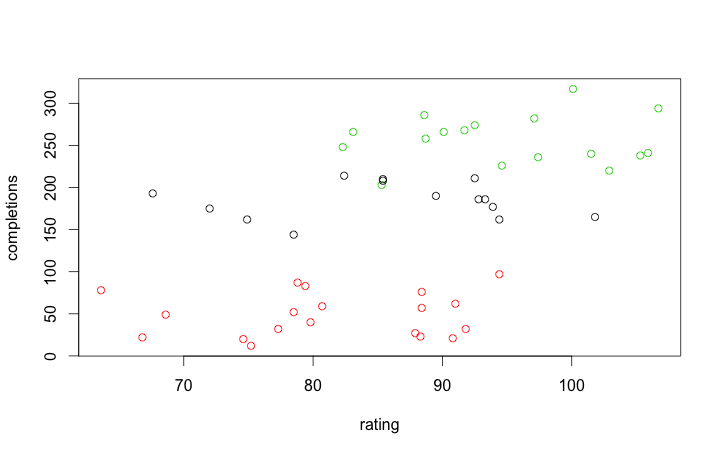
\includegraphics[width=8cm]{completionsVsRating.png}}%
\hfill
\raisebox{-.6\height}{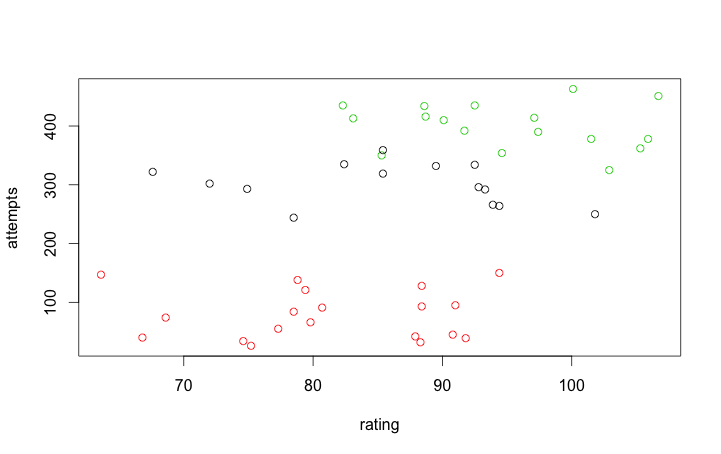
\includegraphics[width=8cm]{attemptsVsRating.png}}%
\par
Finally, looking at how negative stats (Sacks and Interceptions) correlate with ranking. One really interesting find is that Sacks as they relate to the top tier, is that the top tier gets sacked more than the other groups--especially more than group 3. This seems to hold mostly true with interceptions as well:
\par
\raisebox{-.6\height}{
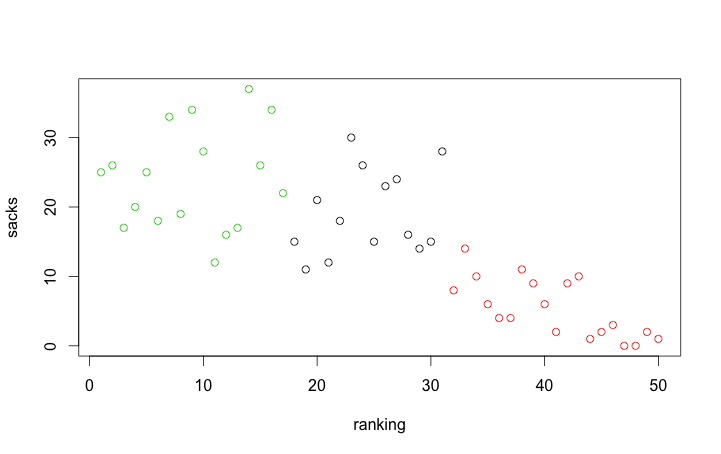
\includegraphics[width=8cm]{sacksVsRanking.png}}%
\hfill
\raisebox{-.6\height}{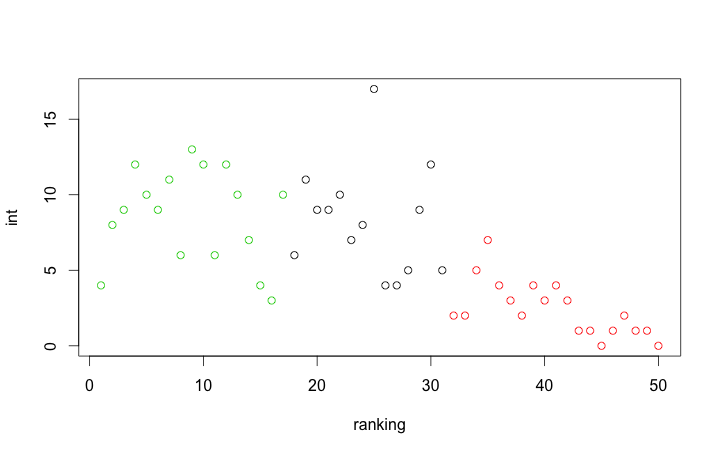
\includegraphics[width=8cm]{intVsRanking.png}}%
\par
Considering that the ranking is based on number of yards, I suppose this makes some sense as to get a lot of yards a player needs to play a lot of time, therefore increasing the chances of sacks and interceptions. 

\subsection*{References}
Epstein, David. n.d. Retrieved from https://www.ics.uci.edu/~eppstein/280/cluster.html
Mathworks.com, 2015. Retrieved from http://www.mathworks.com/discovery/unsupervised-learning.html
NFL.com, 2015. Retrieved from http://www.nfl.com
\end{document}
